% Chapter 1

\chapter{Introducción general} % Main chapter title

\label{Chapter1} % For referencing the chapter elsewhere, use \ref{Chapter1} 
\label{IntroGeneral}


%----------------------------------------------------------------------------------------

% Define some commands to keep the formatting separated from the content 
\newcommand{\keyword}[1]{\textbf{#1}}
\newcommand{\tabhead}[1]{\textbf{#1}}
\newcommand{\code}[1]{\texttt{#1}}
\newcommand{\file}[1]{\texttt{\bfseries#1}}
\newcommand{\option}[1]{\texttt{\itshape#1}}
\newcommand{\grados}{$^{\circ}$}

%----------------------------------------------------------------------------------------

%\section{Introducción}
En este capítulo se realiza una introducción a los conceptos básicos del aprendizaje automático y de conceptos financieros. Asimismo, se menciona el estado del arte en bureau de crédito, y por último se explica la motivación, alcance y objetivos del presente trabajo.  
%----------------------------------------------------------------------------------------
\section{Inteligencia artificial en el ámbito financiero}

El sector financiero fue y sigue siendo uno de los pioneros a la hora de implementar inteligencia artificial, una de las tecnologías más revolucionarias de los últimos tiempos.
La inteligencia artificial se refiere a sistemas o máquinas que imitan la inteligencia humana para realizar tareas, mejorando iterativamente a partir de la información que recopilan. Su objetivo es mejorar significativamente las capacidades humanas. 
Actualmente  la inteligencia artificial mejora el rendimiento y la productividad de las empresas mediante la automatización de los procesos y tareas que antes requerían esfuerzo humano o expertos dedicados a ello.
Hoy en día, muchas aplicaciones de inteligencia artificial son utilizadas tanto por instituciones tradicionales como por fintech. Un score crediticio que utiliza inteligencia artificial es mucho mas completo y sofisticado comparado con criterios tradicionales de score de crédito.
El score o scoring es un método estadístico para predecir comportamientos futuros. Asigna un número de tres cifras que también puede ser determinado como un porcentaje de probabilidad de ocurrencia de un evento futuro y es uno de los factores que analizan los prestamistas ante solicitudes de crédito.  
Los bancos digitales y fintech utilizan algoritmos de aprendizaje automático o machine learning cuya importancia radica en la objetividad y la eliminación de sesgos para la toma de decisiones. Asimismo, la capacidad de cómputo de este tipo de sistemas, permite manejar grandes cantidades de datos en poco tiempo y la computación cognitiva ayuda a administrar datos estructurados y no estructurados. Los algoritmos analizan historiales de transacciones e identifican a tiempo signos de futuros problemas.

%\subsection{Una introducción (no tan corta) a \LaTeX{}}

%\subsubsection{Una subsubsección}

%\subsection{Guía matemática rápida para \LaTeX{}}


%----------------------------------------------------------------------------------------

\section{Estado del arte: caso Nosis}

Nosis es una empresa fundada en la década del 80 con el objeto de brindar información de antecedentes comerciales, 
mercados financieros en línea y comercio exterior para aportar herramientas analíticas que faciliten la toma de decisiones.
Como bureau, cuenta con bases de datos exclusivas, información compartida por mas de 100 entidades, información pública tanto del BCRA,ANSES, AFIP, entre otros  e innovadoras técnicas analíicas con actualización constante de datos. Una de sus principales unidades de negocio hace referencia a los informes comerciales que tienen como variable principal el score desarrollado por la misma empresa. El score de nosis es un ejemplo de un score de riesgo. Logra ordenar y predecir de forma eficiente comportamientos en distintas circunstancias. 
Brinda información sobre la probabilidad de default o mora del cliente consultado desde el momento de la consulta y 12 meses hacia adelante. Detrás de este número único o calificación, hay mas de 70 variables de información dentro del algoritmo desarrollado por la empresa, que puso en consideración el endeudamiento historico de varias fuentes de información y mas de 600 atributos de datos. El algoritmo se procesa en el momento de la consulta e indica que cuanto más alto sea el score, existe una menor probabilidad de default o mora.  
Las bases de datos con las que cuenta Nosis, cubren el 99.99\% del endeudamiento de una persona o empresa con el sistema financiero total a nivel país. 




%----------------------------------------------------------------------------------------

\section{Motivación}

%\subsection{Carpetas}

La principal motivación para la realización de este trabajo, fue la eliminación de subjetividades en procesos de asignación de límite crediticio, la reducción de la deuda generada por los clientes y el mayor aprovechamiento del presupuesto destinado al otorgamiento de créditos, junto a la adopción de tecnologías relacionadas al análisis predictivo en una empresa tradicional con muchos años en el mercado y con procesos establecidos adversos al cambio.
El presente trabajo fue el primer algoritmo desarrollado por el área de data analytics y el principal caso de uso dentro de la compañía, rompiendo así la brecha entre las distintas áreas de negocio y de TI (tecnología de la información).


%----------------------------------------------------------------------------------------

\section{Objetivos y alcance}

\subsection{Objetivos}

El propósito de este trabajo consistió esencialmente en el dise˜ño, pruebas e implementación de una solución de inteligencia artificial que permite estimar la mora
y la rotación del crédito de los clientes activos de la compañía, asegurando a una mejor distribución, teniendo en cuenta distintos aspectos del cliente en cuanto sus compras, pagos atrasados, deuda total vigente, cheques rechazados, antigüedad e historial de pagos, entre otras variables.

En la figura \ref{fig:Diagrama en bloques del sistema}.  se observa un diagrama general de la solución y las etapas que la componen.

\vspace{1cm}

\begin{figure}[htbp]
	\centering
	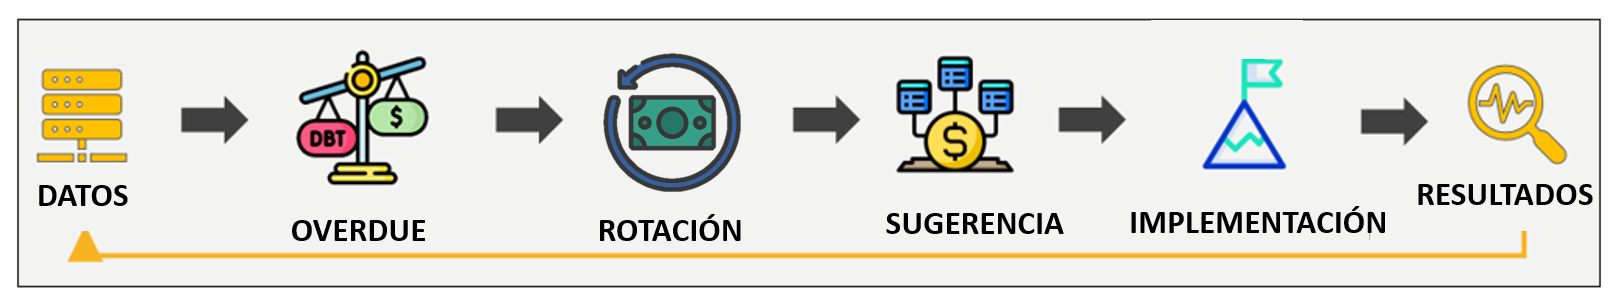
\includegraphics[width=1.0\textwidth]{./Figures/Diagrama de FlujoV2.png}
	\caption{Diagrama en bloques del sistema.}
	\label{fig:Diagrama en bloques del sistema}
\end{figure}

\vspace{1cm}

En el capítulo 3 se detalla el diseño y la implementación de las etapas que componen este sistema.



\subsection{Alcance}


El alcance de este trabajo estuvo orientado a desarrollar una solución de software que permite cubrir aspectos que giran en torno a los siguientes ejes:

\begin {enumerate}
\item Entendimiento del problema: 
	\begin {itemize}
	\item Assesment del proceso de asignación manual del límite de
crédito. 
	\item Resultados esperados a partir de la implementación de la solución.
	\end {itemize}

	
\item Aspectos relacionados al entendimiento del negocio: 
	\begin {itemize}
	\item Entendimiento de las restricciones asociadas al proceso. 
	\item Entendimiento de aspectos generales del negocio.
	\end {itemize}
	
\item Aspectos relacionados a la adquisición y comprensión de datos: 
	\begin {itemize}
	\item Assesment de las fuentes de datos (modelos en datawarehouse y otras). 
	\item Exploración de los datos para determinar la calidad de la información.
	\end {itemize}
	
\item Aspectos relacionados al modelado: 
	\begin {itemize}
	\item Diseño de características: generación de variables adicionales a partir de los datos sin procesar para facilitar 
el entrenamiento del modelo.
	\item Entrenamiento del modelo: elección del modelo que responda a la pregunta de negocio con la máxima precisión, evaluando métricas de éxito.
	\end {itemize}
	
\item Aspectos relacionados al despliegue: 
	\begin {itemize}
	\item Implementación del/los modelo/s en un entorno de producción o similar para el consumo por el usuario final o aplicaciones. 
	\end {itemize}
\end {enumerate}
 
El alcance de este trabajo no abarcó:
\begin {itemize}
\item El mantenimiento de la base de datos en la cual se aloja la información generadora de la entrada para el modelo de inteligencia artificial.
\item La instalación y mantenimiento del hardware necesario para el procesamiento de información del modelo desarrollado.
\item La disponibilización de la salida del algoritmo directamente en alguna aplicación de la compañía
\end {itemize}